\documentclass[10pt]{beamer}
\usepackage{blindtext}
\usepackage{enumitem}
\usepackage{xcolor}
\usepackage{graphicx} 
\usepackage{tikz}
\usepackage{ragged2e}
\usetikzlibrary{er,positioning}
\usetheme{CambridgeUS}


\title{RPI Case Presentation}
\subtitle{ECO 4934 \\ Topics in Econometrics \\ Summer C, 2024}
\author{Group B: Jonathon Lewis \\ Python Irvin \\ Alexis Leclerc \\ Polina Baikova}

\begin{document}
	
\begin{frame}
\titlepage
\end{frame}
	
	
\begin{frame}[t]{Problem Description}\justifying \vspace{20pt}
	In continuous software engineering, each major release introduces significant new or modified functionality. Developers strive to resolve as many bugs as possible. Analyzing bug reports leverages extensive data from defect tracking systems to gain valuable insights into the bug triaging process.
	\vskip 16pt
	In this case we will use The Eclipse and Mozilla Defect Tracking Dataset. We will focus on analyzing the Eclipse subset. The task is to explore the dataset to develop insights into the factors that affect the likelihood of a bug being fixed. The goal is then to develop a prediction model for which bugs would be fixed.
	
\end{frame}


\begin{frame}[t]{Problem Description}\justifying \vspace{2pt}
	Our main objective is to develop prediction model using machine learning techniques including logistic regression, logistic regression with LASSO regularization, random forest, bagging, and boosting.  
	
	Given the dataset’s complexity, the following steps will be implemented to complete the task: 
	\begin{description}[font=$\bullet$~\normalfont\scshape\color{red!50!black}]
		\item [Exploratory Data Analysis:] Understanding the dataset and identifying key factors influencing bug resolution.
		\item [Feature Engineering:] Creating relevant variables that could impact the likelihood of bug resolution.
		\item [Model Development:] Building and evaluating models, tuning the parameters. 
		\item [Model Predictions:] Applying the developed models to a hold-out dataset to predict bug fixes.
		
	\end{description}
\end{frame}


\begin{frame}[t]{Data}\justifying \vspace{20pt}
	The Eclipse dataset provided for this analysis includes twelve CSV files: the reports file, that includes the two report attributes are unchangeable: the reporter and the opening time of the reported bug, and files with different attributes, each with a list of updates and changes that have been performed during the bug's lifetime.
	\vskip 16pt  
	We used Python to clean, filter and sort the original CSV files. Next, we joined them into a table in one of our MariaDB MySQL Databases.  
\end{frame}


\begin{frame}[t]{Data}\justifying \vspace{10pt}
\begin{figure}[htp]
	\centering
	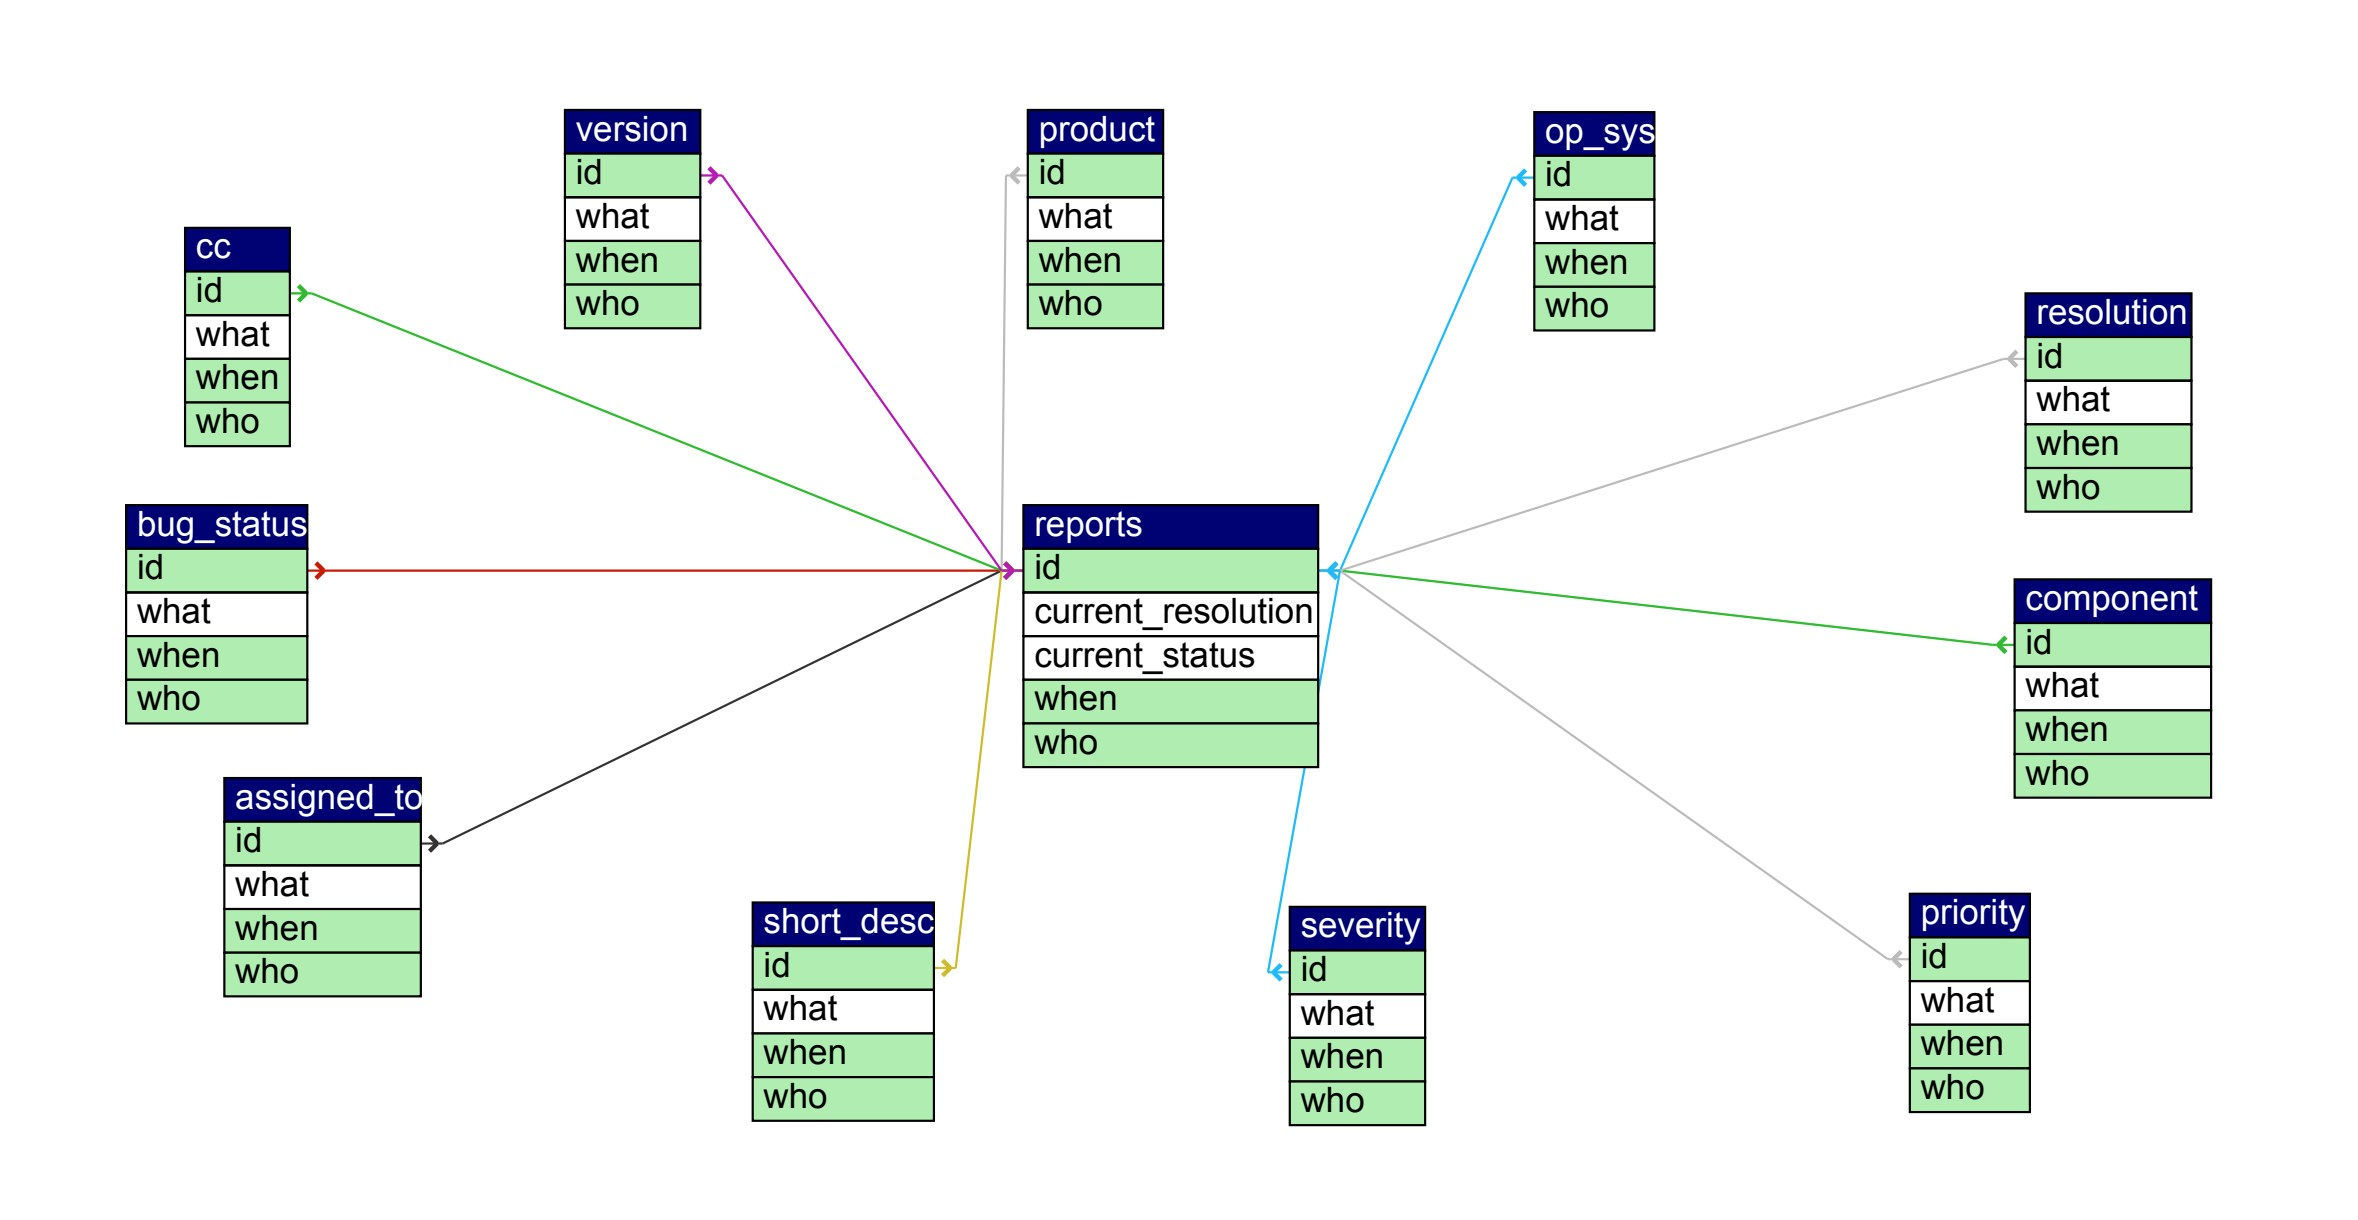
\includegraphics[width=0.9\textwidth]{./ER_diagram.jpg}
	\caption{ER Diagram}
	\label{fig:picture1}
\end{figure}
\end{frame}


\begin{frame}[t]{Data}\justifying \vspace{20pt}
	Our next step was to separate the non-update features (severity, priority, component, \texttt{op\_sys}, who, when, \texttt{current\_status}, \texttt{current\_resolution}, version, product, \texttt{report\_id})into one database and made each category, for each feature, a dummy variable and split/indexed the table into Train, Test and Validation tables. 
	\vskip 10pt 
	We then created another database to calculate and generate additional variables, which included attributes such as reports, resolution, \texttt{bug\_status}, \texttt{assigned\_to}, and \texttt{cc\_email}. These additional variables were merged with the Train, Test, and Validation datasets. Finally, the comprehensive dataset was downloaded as a .dat file for model implementation.
\end{frame}


\begin{frame}[t]{Data}\justifying \vspace{20pt}
	During development we implemented MySQL code in R using RMySQL and DBI libraries, that connected to the database, pulling the data into the R environment while excluding one dummy for each category to prevent multicollinearity and removed features containing less than 3 successes. (resembling a data pipeline). This was done to facilitate testing our models with different combinations of features. We also excluded versions. We took the schemas of our MariaDB databases and converted them into SQLITE3 databases, which is what we use in the makefile. From there we downloaded the .dat files of the tables to run our regressions. All of the relational databases had a backup to prevent any unexpected event.
\end{frame}


\begin{frame}[t]{Logistic Regression} \justifying \vspace{10pt}
	Logistic regression is a statistical method used when the dependent variable is binary. In our case, the dependent variable is whether a bug will be fixed (1) or not (0).
	
	The logistic regression model can be expressed as:
	\[ logit\left( p\right)=\ln \left( \dfrac{p}{\left( 1-p\right) }\right) =\beta_{0}+\beta _{1}X_{1}+\beta _{2}X_{2}+\ldots +\beta_{n}X_{n} \]
	where:
	\begin{description}[font=$\bullet$~\normalfont\scshape\color{red!50!black}]
	\item p is the probability that the bug will be fixed
	\item $\beta_{0}$ is the intercept term
	\item $\beta_{1}$, $\beta_{2}$, ... $\beta_{n}$ are coefficients for the predictor variables $X_{1}$, $X_{2}$, ... $X_{n}$
	\end{description}
\end{frame}


\begin{frame}[t]{Logistic Regression with LASSO regularization} \justifying \vspace{8pt}
	When combined with Lasso regularization, logistic regression becomes a powerful tool for feature selection and preventing overfitting. Lasso (Least Absolute Shrinkage and Selection Operator) regularization is a technique that adds a penalty equal to the absolute value of the magnitude of coefficients to the loss function. The Lasso regularization term is added to the logistic regression cost function to control the complexity of the model. 
	
	The regularized logistic regression model can be expressed as:
	\[ logit\left( p\right)=\ln \left( \dfrac{p}{\left( 1-p\right) }\right) =\beta_{0}+\beta _{1}X_{1}+\beta _{2}X_{2}+\ldots +\beta_{n}X_{n} +\lambda \sum \left| \beta _{i}\right|\]
	where:
	\begin{description}[font=$\bullet$~\normalfont\scshape\color{red!50!black}]
		\item $\lambda$ is the regularization parameter that controls the amount of shrinkage applied to the coefficients
		\item $\sum \left| \beta _{i}\right|$ is the sum of the absolute values of the coefficients
	\end{description}
\end{frame}


\begin{frame}[t]{Logistic Regression with LASSO regularization} \justifying \vspace{10pt}
	To predict the likelihood of bug resolution, we constructed a LASSO model using the 'glmnet' package. This method allowed us to automatically select the most relevant features by determining the optimal lambda value through cross-validation, effectively reducing model complexity and preventing overfitting. By penalizing less significant predictors, we achieved a more robust and interpretable model, enhancing the accuracy of our predictions for bug resolution likelihood.
	\vskip 16pt 
	The variables selected by LASSO were then subjected to logistic regression with LASSO regularization, specifically trained to predict the $\texttt{current\_resolution\_FIXED}$ status. Predictions were generated for the validation set, and the model's performance was evaluated using ROC analysis.
\end{frame}


\begin{frame}[t]{Logistic Regression with LASSO regularization}\justifying \vspace{1pt}
	\begin{figure}[htp]
		\centering
		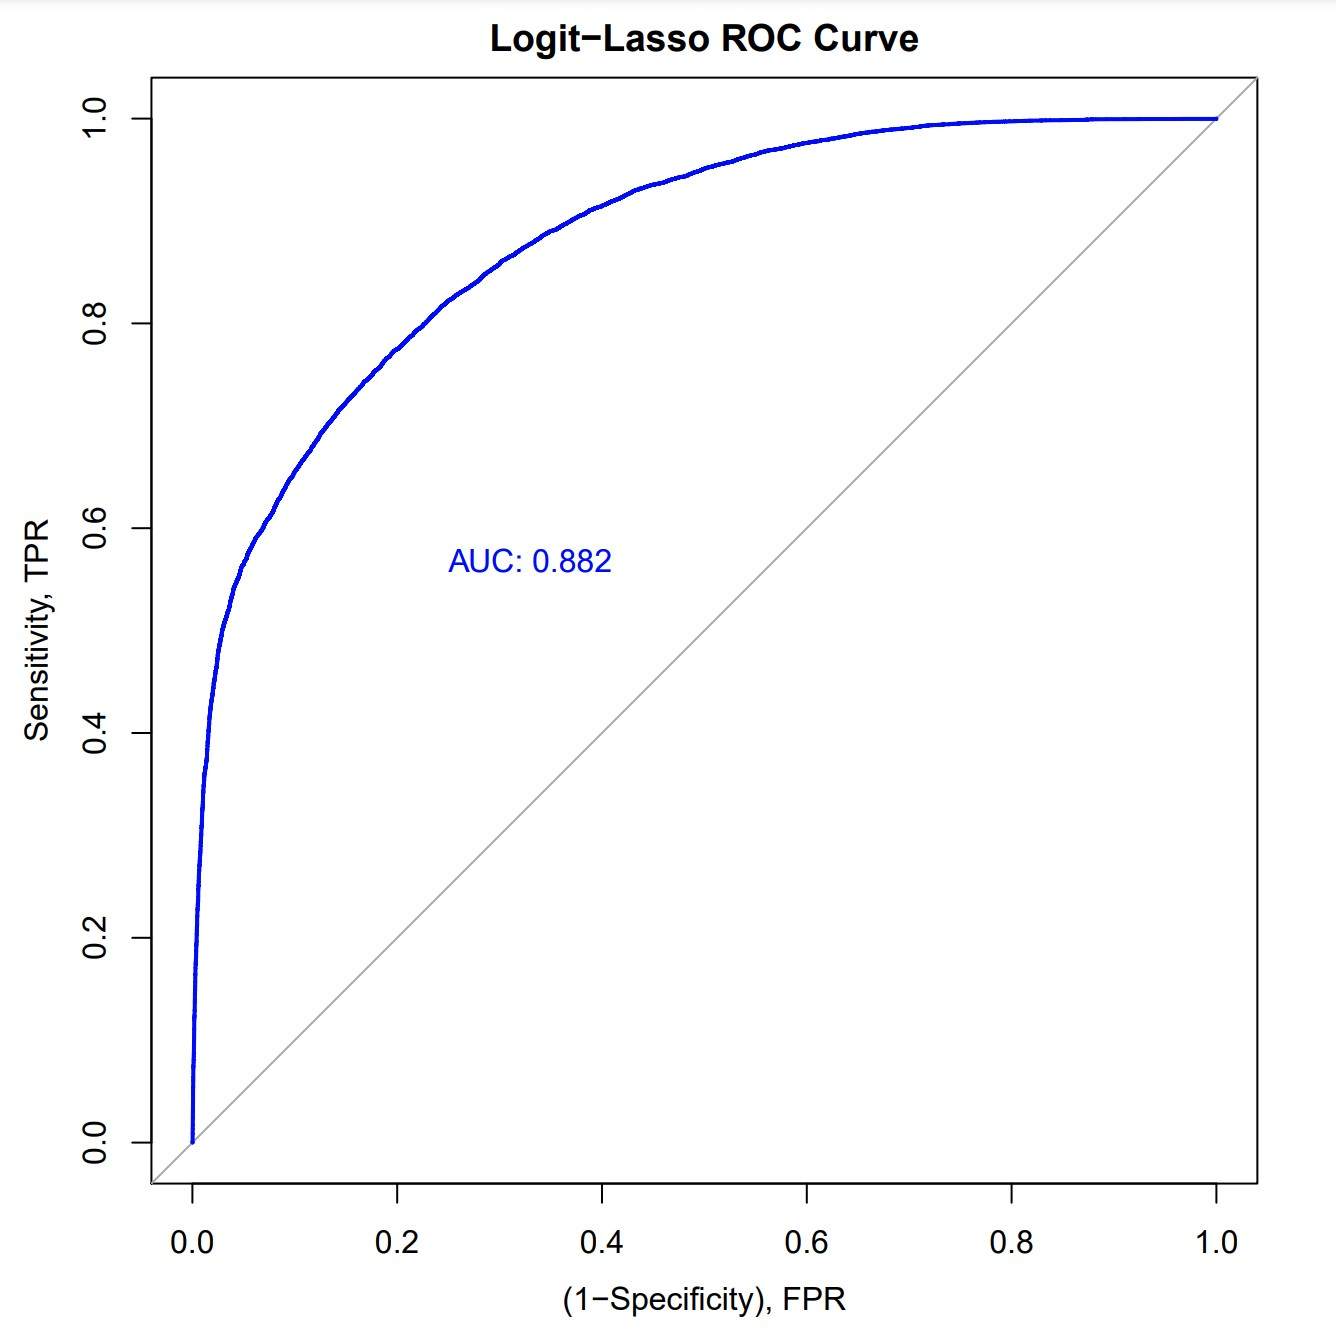
\includegraphics[width=0.54\textwidth]{./Logit-Lasso_ROC.jpg}
		\caption{Logit-LASSO ROC curve}
		\label{fig:picture1}
	\end{figure}
\end{frame}


\begin{frame}[t]{Variables} \justifying \vspace{25pt}
	Our dataset comprised 143,553 observations with 185 features. Initially, we ran our Logit model with 76 features, excluding 19 features for multicollinearity, features containing less than 3 successes, and versions. After running the Lasso-Logit model, the Lasso regression excluded another 3 features. From there  all our models used 73 features consisting of 66 Bernoulli random variables and 6 continuous random variables and 1 discrete random variable. 
	$\texttt{Current\_status}$ and $\texttt{current\_resolution}$ served as the final update of a bug report while $\texttt{bug\_status\_update}$ and $\texttt{resolution\_update}$ contained the bug report edits made from the time the bug was opened to the time the bug was closed. 
\end{frame}


\begin{frame}[t]{Variables} \justifying \vspace{25pt}
	The Continuous Random Variables:
	\begin{enumerate}
	\item [1.] Our first variable measures the Average Success Rate of the aggregated Bug Assignees for each unique bug report id.
	\item [2.] Our second variable measures the Average Success Rate of each Bug Reporter for all bug reports.
	\item [3.] Our third variable measures the Reputation of each Bug Reporter, calculated by multiplying the The Success Rate of each Bug Reporter by the Log of Total Bug Reports for the corresponding Bug Reporter.
	\item [4.] Our fourth variable measures the proportion of edits for each unique existing bug reporter for each bug report id multiplied by the bug reporters reputation.
	\item [5.] Our fifth variable measures the length of time the bug report was open. 
	\end{enumerate}
\end{frame}


\begin{frame}[t]{Decision Tree}\justifying \vspace{10pt}
	A decision tree is a supervised learning algorithm used for classification and regression tasks. It splits the dataset into subsets based on the most significant feature at each node, forming a tree-like structure of decisions. Internal nodes represent tests on attributes, branches represent outcomes, and leaf nodes represent class labels or continuous values. 
	\vskip 8pt
	We constructed a decision tree model to predict the likelihood of a bug being fixed using the rpart package. The model was trained on the training dataset without pruning (cp = 0). Predictions were made in parallel for the validation set using the foreach package to improve computational efficiency. The predicted probabilities for the positive class were then evaluated using ROC analysis to assess the model's performance.
\end{frame}


\begin{frame}[t]{Decision Tree}\justifying \vspace{1pt}
	\begin{figure}[htp]
		\centering
		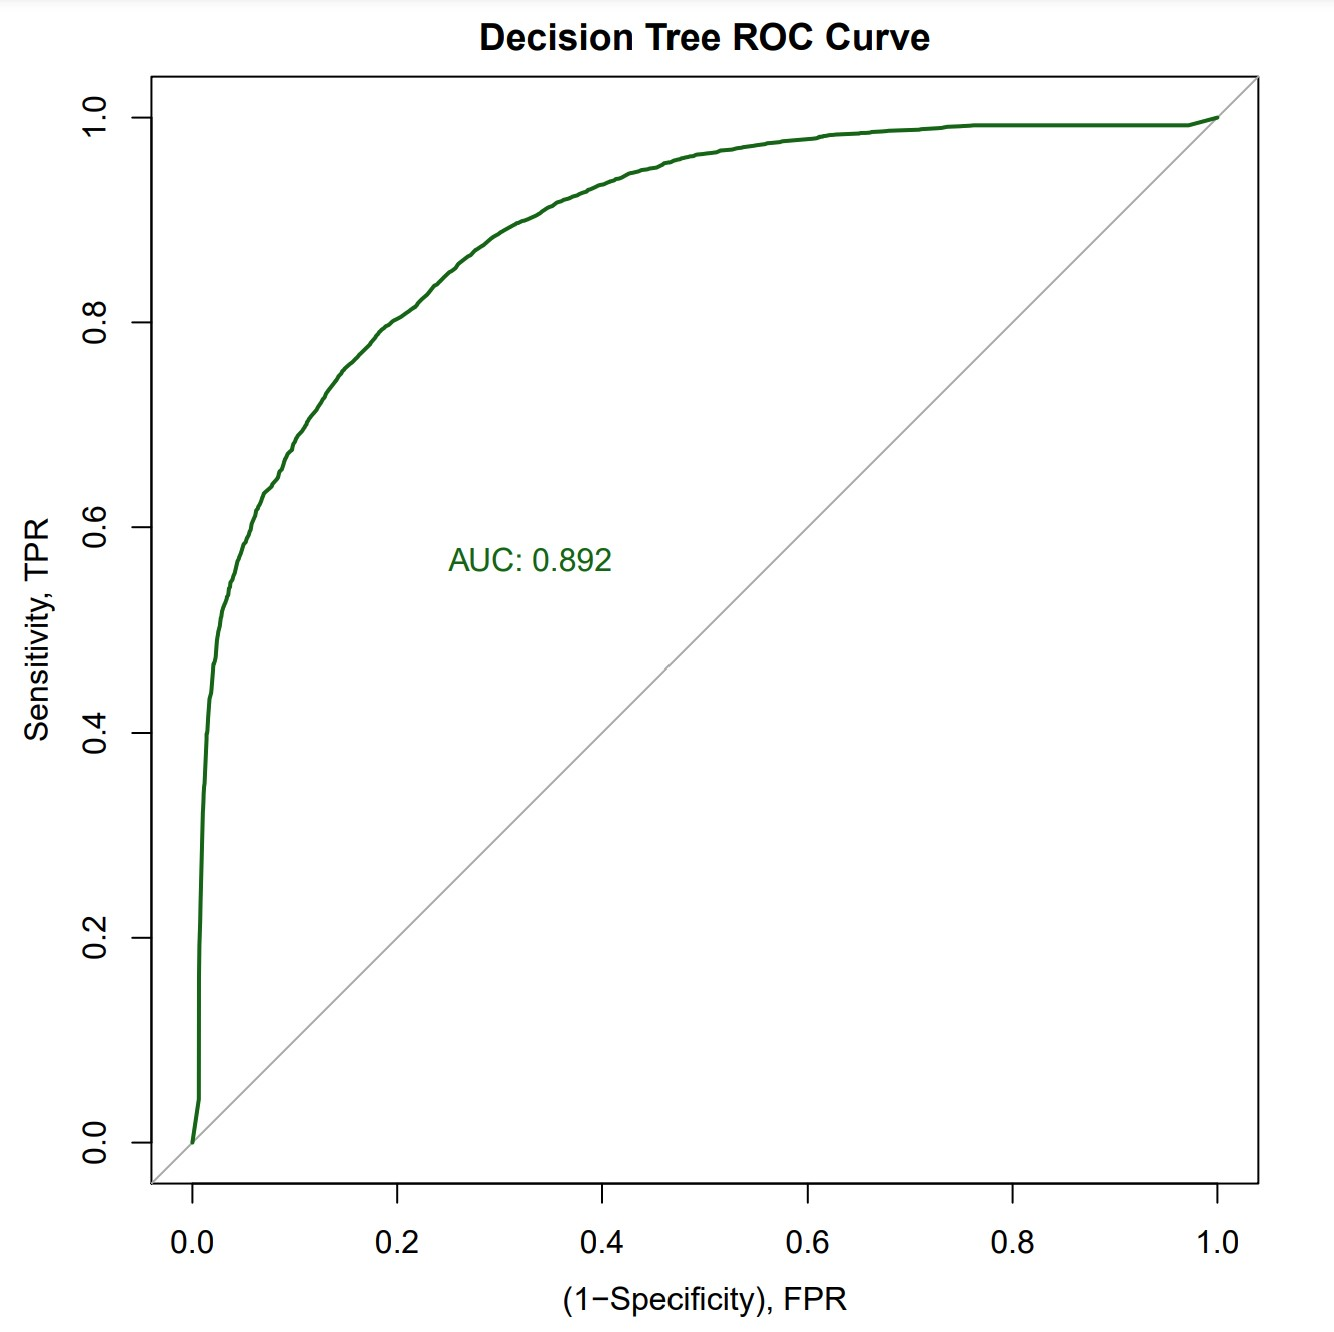
\includegraphics[width=0.54\textwidth]{./Decision_tree_ROC.jpg}
		\caption{Decision Tree ROC curve}
		\label{fig:picture1}
	\end{figure}
\end{frame}


\begin{frame}[t]{Random Forest}\justifying \vspace{10pt}
	Random Forest is an ensemble learning method that improves predictive performance by combining multiple decision trees. It is particularly effective in predicting whether a software bug will be fixed, based on various characteristics of the bug report. Each tree in the forest is trained on a bootstrap sample of the data with random feature selection at each node. This method reduces variance, mitigates overfitting, and provides feature importance insights, improving prediction reliability.
	\vskip 8pt
	We developed a custom random forest model to predict bug resolution likelihood. The model was built using 1000 decision trees, each trained on bootstrap samples of the training data with a random selection of 10 features per tree. Predictions for the validation set were aggregated through majority voting from all the individual trees.
\end{frame}


\begin{frame}[t]{Random Forest}\justifying \vspace{1pt}
	\begin{figure}[htp]
		\centering
		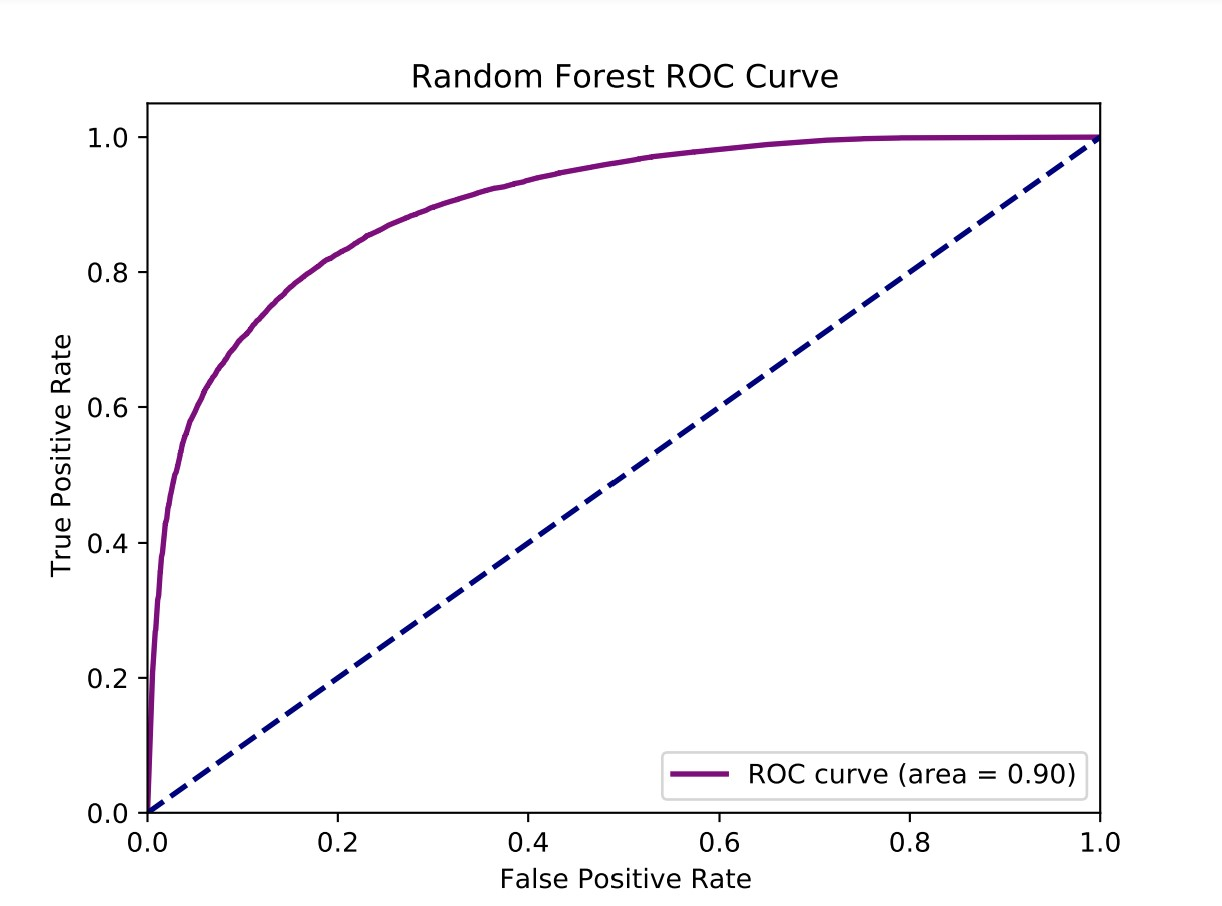
\includegraphics[width=0.7\textwidth]{./Random_forest_ROC.jpg}
		\caption{Decision Tree ROC curve}
		\label{fig:picture1}
	\end{figure}
\end{frame}
 
 
\begin{frame}[t]{Bagging}\justifying \vspace{10pt}
	Bagging, or Bootstrap Aggregating, is an ensemble learning technique that enhances the accuracy and stability of machine learning models by reducing variance. It involves creating multiple decision trees from different bootstrap samples of the training data and combining their predictions. This method improves model robustness to outliers and noise. By leveraging multiple models, bagging produces more accurate and reliable predictions.
	\vskip 8pt
	A bagging model was constructed using the treebag method from the 'caret' package. The model training involved 5-fold cross-validation, allowing for parallel processing to enhance performance. After training, predictions for the validation set were generated, focusing on the probability of the positive class. 
\end{frame}


\begin{frame}[t]{Bagging}\justifying \vspace{1pt}
	\begin{figure}[htp]
		\centering
		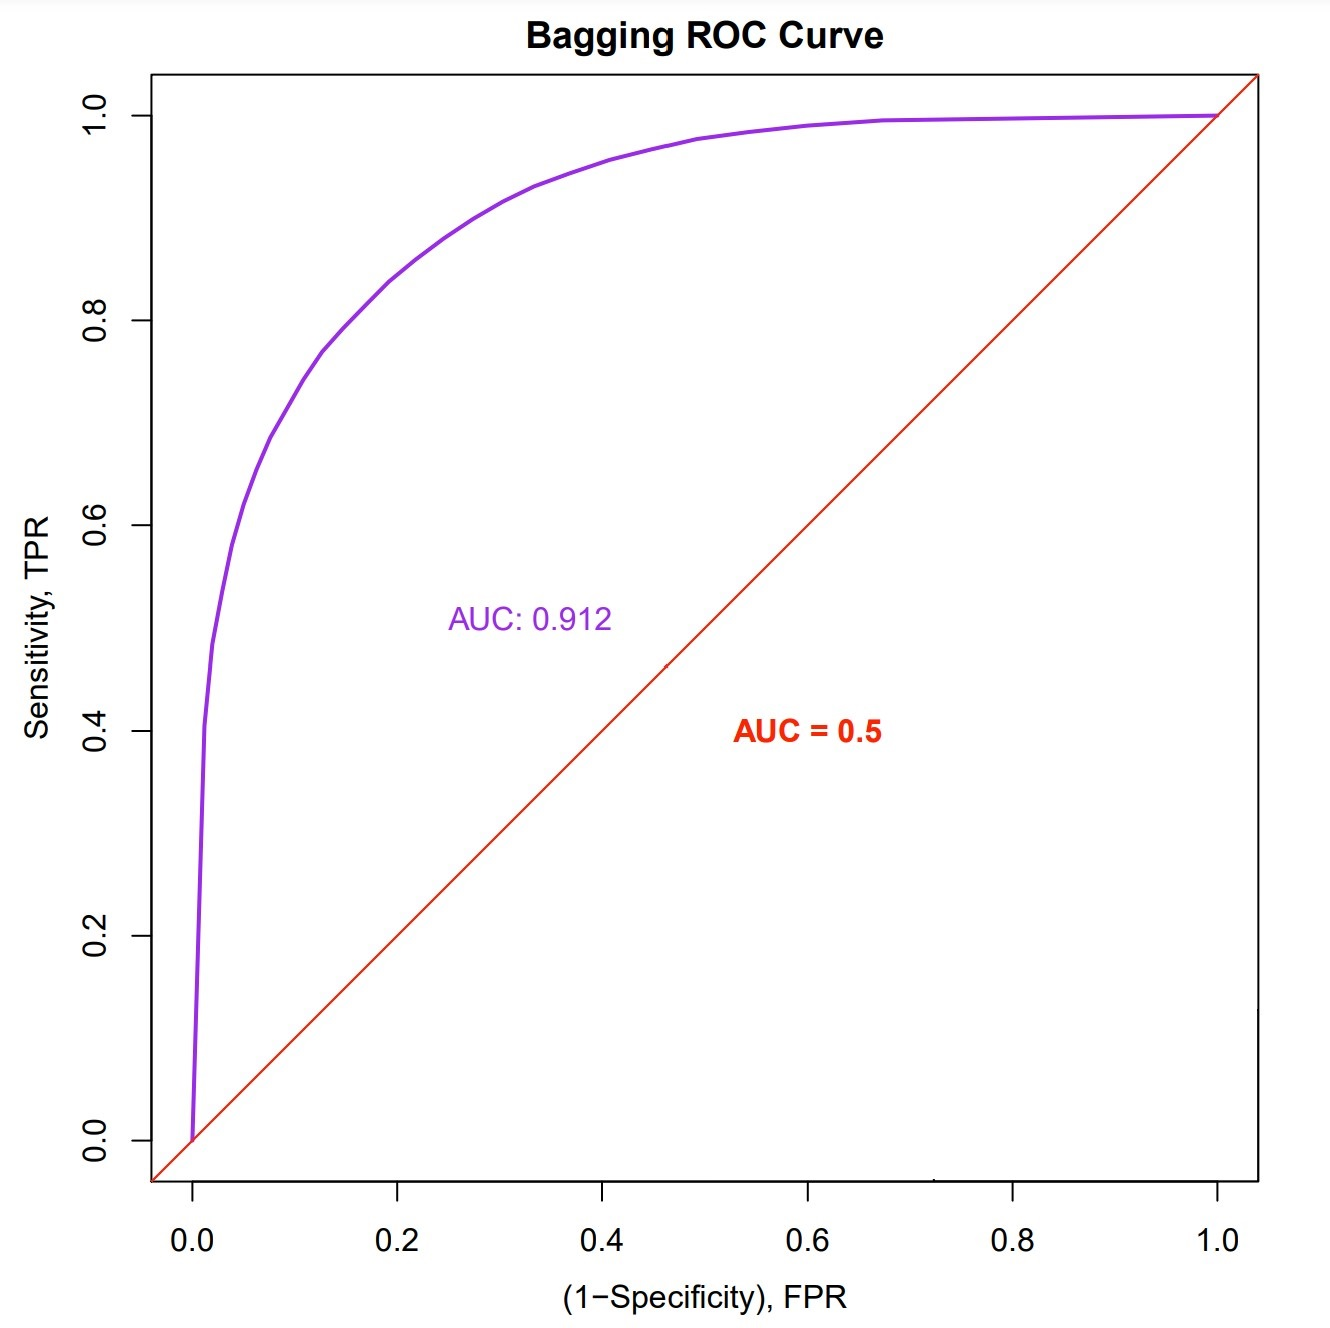
\includegraphics[width=0.54\textwidth]{./Bagging_ROC.jpg}
		\caption{Bagging ROC curve}
		\label{fig:picture1}
	\end{figure}
\end{frame}


\begin{frame}[t]{Boosting}\justifying \vspace{10pt}
	Boosting is an ensemble learning technique that improves the accuracy and robustness of predictive models by combining several base models sequentially, each correcting the errors of its predecessor. In the context of software bug reports, boosting can predict whether a bug will be fixed by focusing on misclassified instances and iteratively training new models. 
	\vskip 8pt
	We implemented a boosting model using the gbm package. Boosting involves training multiple weak learners sequentially, each trying to correct the errors of its predecessor. We set specific parameters for the boosting process, including the number of trees (n.trees = 10000), interaction depth (interaction.depth = 3), shrinkage rate (shrinkage = 0.01), and subsampling rate (bag.fraction = 0.5).
\end{frame}

\begin{frame}[t]{Boosting}\justifying \vspace{0pt}
	\begin{figure}[htp]
		\centering
		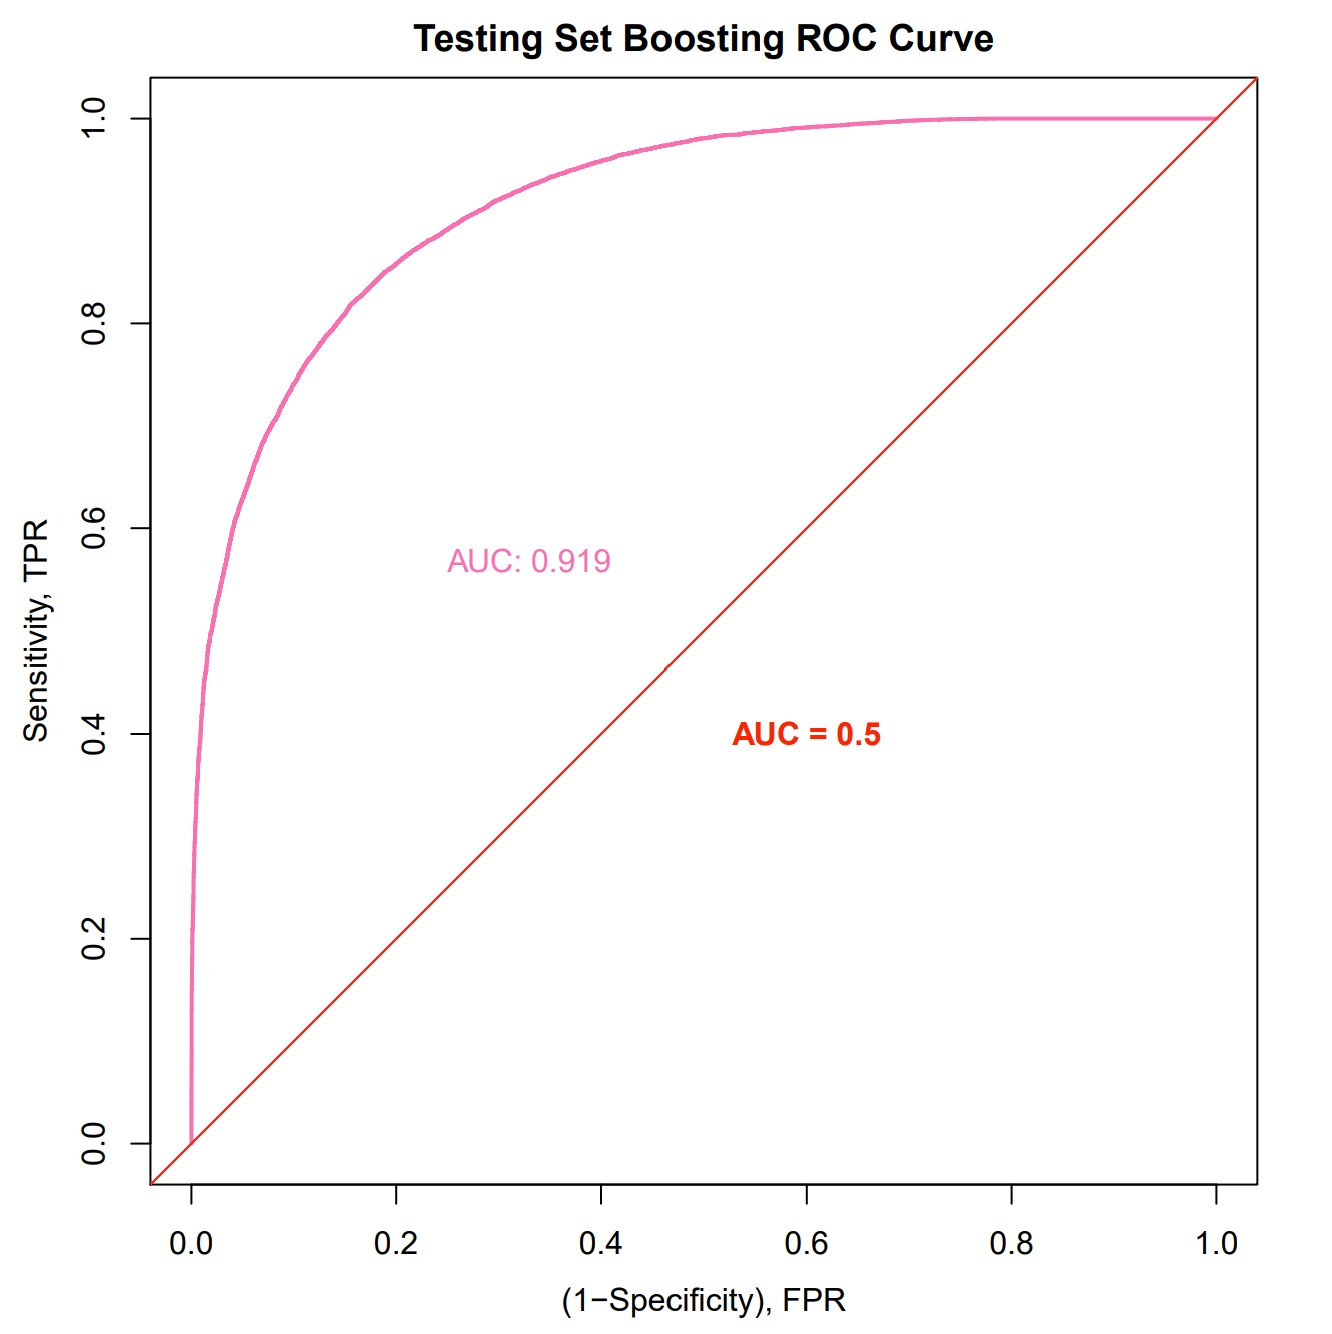
\includegraphics[width=0.54\textwidth]{./Boosting_ROC.jpg}
		\caption{Boosting ROC curve}
		\label{fig:picture1}
	\end{figure}
\end{frame}


\begin{frame}[t]{Results}\justifying \vspace{10pt}
The ROC curve analysis compares the performance of four predictive models: Logit-Lasso, Decision Tree, Bagging, and Boosting, in predicting bug resolution. Boosting outperformed all models with the highest AUC of 0.915, indicating its superior predictive power by iteratively refining predictions. Bagging followed with an AUC of 0.898, enhancing model stability through averaging multiple decision trees. The Decision Tree model achieved an AUC of 0.893, performing well but slightly less robust than the ensemble methods. Logit-Lasso had the lowest AUC of 0.881, providing solid but less effective predictions due to its linear nature. 
\end{frame}


\begin{frame}[t]{Results}\justifying \vspace{1pt}
	\begin{figure}[htp]
		\centering
		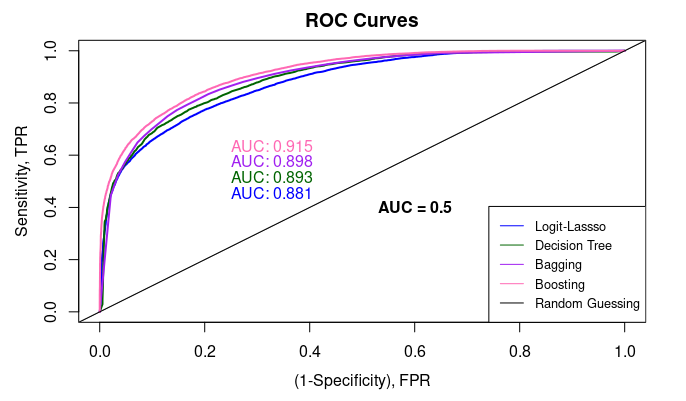
\includegraphics[width=0.8\textwidth]{./MemoCurve.png}
		\caption{ROC curves for Logit-LASSO, Decision Tree, Bagging, and Boosting}
		\label{fig:picture1}
	\end{figure}
\end{frame}

\end{document}